\documentclass[12pt]{article}
\usepackage{graphicx}
\usepackage{amsmath}
\usepackage{amssymb}
\usepackage{hyperref}
\usepackage{listings}
\usepackage{xcolor}
\usepackage{pgfplots}
\usepackage{pgfplotstable}
\usepackage{pgffor}
\usepackage{verbatim}
\usepackage[a4paper, margin=1in]{geometry}

% Define colors for code only
\definecolor{codebg}{rgb}{0.9, 0.9, 0.9}
\definecolor{commentgreen}{rgb}{0, 0.6, 0}
\definecolor{keywordblue}{rgb}{0, 0, 1}
\definecolor{stringred}{rgb}{0.8, 0, 0}

\lstdefinestyle{customc}{
    backgroundcolor=\color{codebg},
    commentstyle=\color{commentgreen},
    keywordstyle=\color{keywordblue},
    stringstyle=\color{stringred},
    basicstyle=\ttfamily\footnotesize,
    breakatwhitespace=false,
    breaklines=true,
    captionpos=b,
    keepspaces=true,
    numbers=left,
    numbersep=5pt,
    numberstyle=\tiny\color{gray},
    showspaces=false,
    showstringspaces=false,
    showtabs=false,
    tabsize=2
}

\title{Benchmark Suite: Matrix-Matrix Multiplication (mmult)}
\author{Mohammed Mansour}
\date{\today}

\begin{document}

\maketitle

\section{Introduction}
Matrix-matrix multiplication (mmult) is a fundamental operation in scientific computing, machine learning, and computer architecture. This report documents the implementation and evaluation of the mmult benchmark in the YABMS benchmark suite. The objective is to understand the performance characteristics of different datasets and analyze the impact of various optimization techniques.

\section{Collaboration}
I discussed the details of the project with Moneer Al-Bokhaiti. We covered the project requirements, the necessary tools, and the complexity of the code. He suggested creating a separate application to generate the dataset. We also agreed that storing the dataset in a binary file would be more efficient than saving it as ASCII text.

Additionally, I attended a meeting conducted by class students, where we discussed various issues related to the project. During this meeting, we broke the implementation into smaller steps to make the development process more manageable.

\section{Naïve Implementation}
The naïve implementation is a simple three-loop to compute the matrix product:
\lstinputlisting[language=C, style=customc, caption=Naïve mmult implementation]{resources/naive_implementation.c}

This method is straightforward but inefficient due to cache misses and redundant memory accesses. Each element of the matrices is accessed multiple times, leading to poor utilization of the CPU cache. Additionally, the lack of optimization techniques such as loop unrolling results in nonoptimal performance, especially for larger datasets.

\subsection{Dataset Generation}
The dataset required for the benchmark is generated using a Python script. The script generates random matrices, performs matrix multiplication, and saves the datasets in binary format. The dataset consists of predefined matrix sizes categorized into five sets: testing, small, medium, large, and native.

The following Python script is used for dataset generation:
\lstinputlisting[language=Python, style=customc, caption=Dataset Generation Script]{resources/ds_generator.py}

This script ensures efficient dataset generation by leveraging NumPy for matrix operations and storing the results in a structured binary format. The metadata file provides dimensions for easy retrieval and compatibility with benchmarking implementations.

\section{Evaluation}
The performance of the naïve implementation was evaluated using various dataset sizes. Execution time was measured for each case, and results were compared with optimized implementations.

\subsection{Experimental Setup}
The experiments were conducted on \textbf{Personal Laptop} with the following setup:
\begin{itemize}
    \item Runner Type: Ubuntu-24.04.1 LTS
    \item Operating System: Linux
    \item Processor (CPU): AMD PRO A12-9800B R7, 12 COMPUTE CORES 4C+8G
    \item Memory (RAM): 8 GB
    \item Storage (SSD): 512 GB
    \item Architecture: x64
    \item Compiler: GCC 13.3.0 with optimization flags -O3
\end{itemize}

\subsection{Results}
Table \ref{tab:results} summarizes the execution times for different dataset sizes.

\begin{table}[h]
    \begin{tabular}{|c|c|c|}
        \hline
        \textbf{Dataset Size} & \textbf{Execution Time (ms)} & \textbf{Standard Deviation} \\
        \hline
        Testing (16x8) & 0.005 & 0.0008 \\
        Small (121x115) & 12.137 & 1.189 \\
        Medium (550x480) & 984.68 & 20.159 \\
        Large (962x1221) & 11167 & 46.958 \\
        Native (2500x2100) & 111219 & 661.744 \\
        \hline
    \end{tabular}
        \caption{Execution times for different dataset sizes.}
        \label{tab:results}
    \end{table}

    The benchmark execution logs and results can be accessed at the following link: \url{https://github.com/mohammed0x00/YABMS/tree/main/docs/runtime_data}.

    \newpage
\subsection{Graphical Representation}
The following graph illustrates the execution time versus dataset size for the naïve implementation:
    \begin{center}
        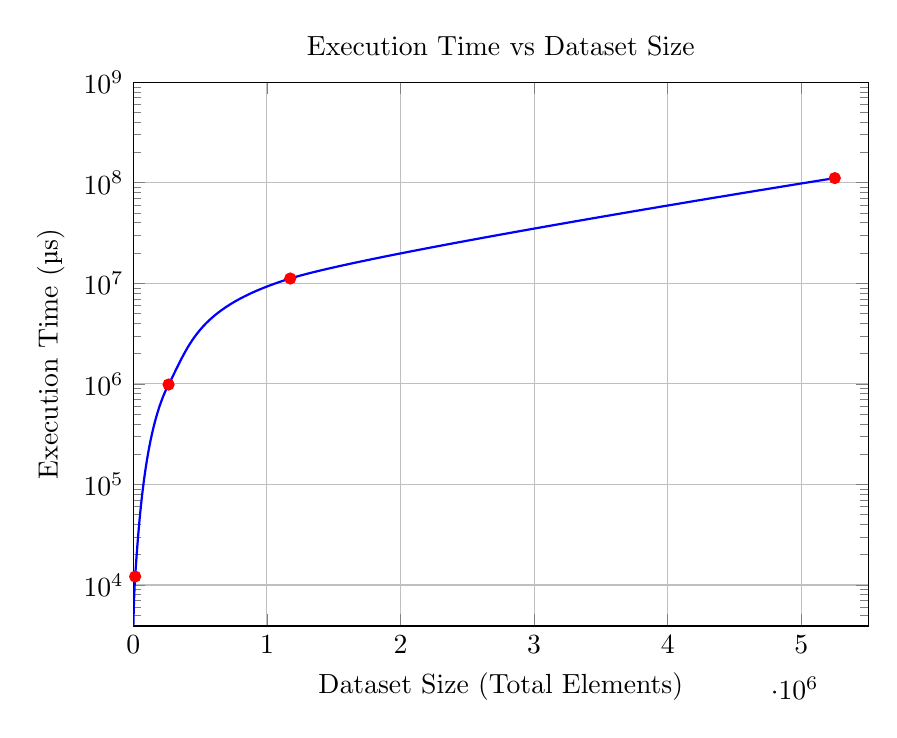
\begin{tikzpicture}
            \begin{axis}[
                ymode=log, % Logarithmic scale for better visualization
                xlabel={Dataset Size (Total Elements)},
                ylabel={Execution Time (µs)},
                title={Execution Time vs Dataset Size},
                width=0.9\textwidth, % Increase width
                height=0.7\textwidth, % Increase height
                xmin=1000, xmax=5500000, % Adjust X-axis limits
                ymin=-0.5, ymax=1e9, % Adjust Y-axis limits
                grid=major
            ]
                % Add smooth curve fitting the points
                \addplot[smooth, thick, blue] coordinates {
                    (128, 5.110)
                    (13915, 12137)
                    (264000, 984676)
                    (1174602, 11166648)
                    (5250000, 111218584)
                };
                
                % Add actual data points
                \addplot[
                    only marks,
                    mark=*,
                    red
                ] coordinates {
                    (128, 5.110)
                    (13915, 12137)
                    (264000, 984676)
                    (1174602, 11166648)
                    (5250000, 111218584)
                };
            \end{axis}
        \end{tikzpicture}
    \end{center}

    \subsection{Detailed Results}
    The execution times for different dataset sizes, measured in milliseconds (ms), along with their standard deviations. As dataset size increases, execution time rises significantly. The "Testing" dataset (16×8), has an execution time of only 0.005 ms with a negligible standard deviation of 0.0008. The "Small" dataset (121×115) takes 12.137 ms, with a slightly higher deviation of 1.189. The "Medium" dataset (550×480) requires around 1 second, showing a noticeable jump in both execution time and deviation (20.159). The "Large" dataset (962×1221) exhibits a much higher execution time of 11 seconds with a deviation of 46.958. Finally, the "Native" dataset (2500×2100) has the highest execution time of 111 seconds and the highest standard deviation of 661.744, indicating increased variability in execution time as dataset size grows.
    \newline \newline
    The detailed results for each dataset size are presented below:
\foreach \dataset in {Testing, Small, Medium, Large, Native} {
    \newpage
    \subsection{\dataset \space Dataset Details}
    The following are the detailed results for the \dataset \space dataset:

    \begin{center}
        \includegraphics[width=0.8\textwidth]{runtime_data/\dataset.png}
    \end{center}

    \lstinputlisting[style=customc, caption=\dataset \space Dataset Output]{runtime_data/\dataset_output.txt}
}






\section{Conclusion}
The benchmarking results demonstrate significant differences in execution times across dataset sizes. The testing dataset (50x50) runs almost instantaneously, whereas the small dataset (121x115) takes 12.137 ms. As matrix sizes increase, execution times rise considerably, with the medium dataset (550x480) requiring 984.676 ms, and the large dataset (962x1221) running for 11.166 seconds. The standard deviation values indicate varying levels of runtime consistency and with larger datasets, it shows greater fluctuation.

These results highlight the inefficiencies of the naïve implementation, especially for larger datasets where cache inefficiencies and memory access patterns significantly impact performance. Future optimizations should focus on improving parallelization and cache optimization.

\section{References}
\begin{enumerate}
    \item GNU Make Manual: \url{https://www.gnu.org/software/make/manual/make.html}
    \item IEEE POSIX Standard: \url{https://ieeexplore.ieee.org/servlet/opac?punumber=6880749}
    \item YABMS Original Repository: \url{https://github.com/hawajkm/YABMS}
    \item YABMS Forked Repository: \url{https://github.com/mohammed0x00/YABMS}
\end{enumerate}

\end{document}
